\subsubsection{Multilayer Perceptron}
\label{sec:mlp-multilayer-perceptron}
A multilayer perceptron consists of multiple perceptrons arranged into layers and solves complex tasks \cite{Bishop1995}.
It is a universal approximator for every function \cite{Cybenko1989} regardless of the activation functions used \cite{Hornik1991}.
Because of the multiple layers and the non-linear activation functions non-linearity is introduced into the network.
Thus, it can distinguish data that is not linearly separable.

There are at least $L=3$ layers.
Each layer contains several perceptrons that are not connected to each other.
However, every perceptron is connected to every perceptron of its subsequent layer.
This type of connection is called a fully-connected network.
Because the data flow within the network is directed, i.e. only in one direction, and acyclic, the architecture is called feedforward neural network.
A visualization of this is shown in \figref{fig:multilayer-perceptron}.
For clarity the weights and biases of each connection and perceptron are not displayed.
\begin{figure}
	\centering
	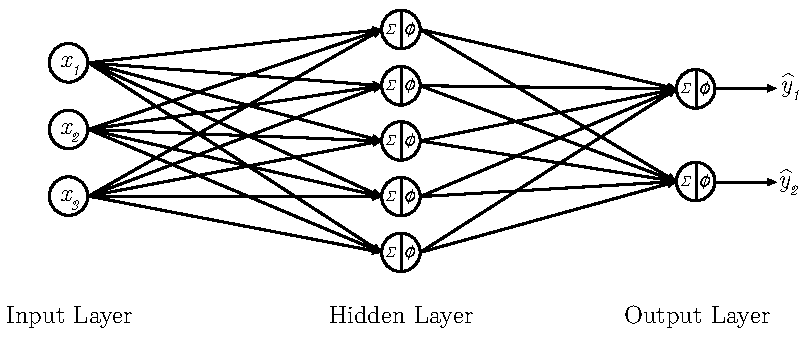
\includegraphics{images/multilayer_perceptron}
	\caption[Multilayer perceptron]{Multilayer perceptron with three layers. Each layer consists of multiple perceptrons. The input layer transfers numeric data into the network. The output layer provides the result of the network for interpretation and further processing. The layers in between, the hidden layers, perform calculations and forward the network data. Each connection between perceptrons has a weight, that is not displayed for clarity. Also, every perceptron has its own bias.}
	\label{fig:multilayer-perceptron}
\end{figure}
Like the single perceptrons every perceptron in the network computes its own activation, a single numerical value, depending on its inputs, weights, and bias.
A specific perceptron is referred to by its layer $l$ and position $j$ within this layer.
Hence, its activation is denoted as $a^{[l]}_{j}$.
Its weight of each connection, called an edge, is denoted as $w^{[l]}_{jk}$ where $k$ is the position of the preceding perceptron in layer $l-1$ and its bias as $b^{[l]}_j$.
All weights of layer $l$ are stored in a compact matrix $\vec{W}^{[l]}$ with each perceptron's weights as a row vector.
In this type of network architecture perceptrons are often referred to as nodes or units.

The input layer serves as an interface for the data.
It does not perform any calculations and just passes the data to the next layer.
The number of perceptrons in this layer depends on the data and how it is prepared.
If the input data is an image, for example, the number of perceptrons should be equal to the number of pixels, so that every perceptron can hold the intensity value of one pixel.
The output layer is responsible for providing the network's computation result so that it can be interpreted and further processed.
The number of perceptrons in this layer depends on the desired number of values.
If types of animals need to be classified in an image, every output perceptron would represent a single type or class, respectively.
Assuming there are three types of animals possible, then there need to be three output perceptrons.
In theory, the perceptron representing the correct class of an animal holds a one and every other a zero if the values are normalized to this range.
Every layer between the input and the output layer is a hidden layer.
Their name comes from the fact that they are not directly accessible from the outside.
Their task is propagating the input data to the output layer while weighting known correlation features more than irrelevant ones.
With at least one hidden layer every continuous function can be approximated.
So, the network models the function 
\begin{equation}
	\label{eq:multilayer-perceptron}
	f(\vec{x}) = \vec{y}
\end{equation}
where
\begin{align}
	\vec{x} &= (x_0, x_1, \cdots, x_{n_x})^T \\
	\vec{y} &= (y_0, y_1, \cdots, y_{n_y})^T
\end{align}
are the input vector with $n_x$ elements and output vector with $n_y$ elements, respectively.

For the next example an image is used again.
The task is to classify a handwritten digit from the MNIST dataset \cite{Lecun98}.
\begin{figure}
	\centering
	\includegraphics[]{images/mnist_digit_3a.png}
	\includegraphics[]{images/mnist_digit_3b.png}
	\caption[Handwritten digits from the MNIST digit dataset]{Handwritten digits from the MNIST digit dataset \cite{Lecun98}. Represented as a $28 \times 28$ pixel matrix. Each cell represents a pixel.}
	\label{fig:mnist-digit}
\end{figure}
The digit can be seen in \figref{fig:mnist-digit}.
Each grid cell represents a pixel.
It is evident that the intensity of every pixel is relevant for classifying the digit.
Thus, every pixel needs an associated perceptron in the input layer of the network.
This real-world data is transferred into the network by flattening the intensity values of the image matrix to a vector.
Therefore, the vector contains $28 \cdot 28 = 784$ elements which equal the number of input perceptrons.
Assuming well-suited weights and biases, that must first be found in practice, the network knows which perceptrons are active for a particular digit.
This means, that if in another image the same or similar pixels or perceptrons, respectively, have high intensities or activations, the same number needs to be classified.
The downside of the flattening is, that the relationship of pixels like their position is lost, which means a loss in overall information.
The consequence of this is, that if a digit has no similar position and shape like the digits the networks know, the classification fails.
If, for example, a digit the network classified correctly is not centered anymore and downscaled to take up only half its original size in a $28 \times 28$ image, completely different perceptrons are active.
Thus, the network cannot find any correlation to the original image or its knowledge of how digits look and returns a wrong classification result.
Another severe downside is the huge number of parameters.
If the image gets larger, the number of input perceptrons naturally needs to be adapted.
Due to this, additional weights and biases are introduced to the network, because every input perceptron is connected to every perceptron of its subsequent layer.
This extends the finding of the optimal weights and biases and needs plenty of resources.
A better solution is provided by convolutional neural networks that are covered in \secref{sec:neural-networks-convolutional-neural-networks}.
